Fuel cells use hydrogen to generate power using a chemical reaction, producing only water and heat as byproducts. This technology does not produce $CO_2$ making it a good candidate to meet the net zero $CO_2$ production goal. The overall challenge to hydrogen production is cost. For cost-competitive transportation hydrogen cost must be comparable to conventional fuels. In order to be competitive, the total  cost of hydrogen needs to be less than \$4/gge. A gge, or gasoline gallon equivalent, is the amount of fuel that has the same amount of energy as a gallon of gasoline. One kilogram of hydrogen is equivalent to one gallon of gasoline \cite{noauthor_hydrogen_nodate}.

Some hydrogen production processes are: 
\begin{description}[font=$\bullet$\scshape\bfseries]
	\item[] Steam-Methane reforming (aka Natural Gas Reforming)
	\item[] Coal Gasification with CCS.
	\item[] High-Temperature Electrolysis.
	\item[] Electrolysis (Solar).
	\item[] Electrolysis (Wind).
\end{description}

The two most common methods for producing hydrogen are steam reforming and electrolysis.
Steam reforming is currently the least expensive way to produce hydrogen. This method separates hydrogen atoms from carbon atoms in methane (CH4). This process results in carbon dioxide emissions.
Electrolysis splits hydrogen from water using an electric current. The emissions are hydrogen and oxygen \cite{noauthor_production_2019}. 

\section{Steam Reforming}

Steam reforming is a mature production process that uses high-temperature steam (700$^{\circ}$C-1000$^{\circ}$C) to produce hydrogen from a methane source. Methane reacts with steam under 3-25 bar pressure in the presence of a catalyst to produce hydrogen, carbon monoxide, and a small portion of carbon dioxide. The reaction is endothermic and requires the supply of heat to occure \cite{noauthor_hydrogen_nodate}.
\begin{equation}
CH_4 + H_2O + heat \rightarrow CO + 3H_2
\end{equation}
A secondary reaction know as water-gas shift reaction occurs producing $CO_2$ and more hydrogen:
\begin{equation}
CO + H_2O \rightarrow CO_2 + H_2
\end{equation}

Even with the upstream process of producing hydrogen from natural gas as well as delivering and storing it for use in fuel cell electric vehicles, the process reduces the greenhouse emissions in half and the use of petroleum over 90\% in today's gasoline vehicles.

\section{Electrolysis}

Electrolysis is the process of using electricity to split water into hydrogen and oxygen, Fig. \ref{fig:electro}. The reaction takes place in a unit called electrolyzer. Electrolyzers consist of an anode and a cathode separated by an electrolyte. Different electrolyzers function in slightly different ways. A few types are polymer electrolyte membrane, alkaline, and solid oxide electrolyzers.

\begin{figure}[H]
	\centering
	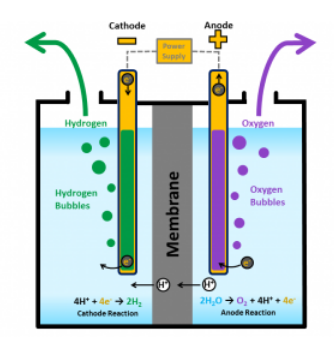
\includegraphics[width=0.4\linewidth]{figures/electrolysis.png}
	\hfill
	\caption{Production of hydrogen by electrolysis.}
	\label{fig:electro}
\end{figure}

Solid oxide electrolyzers must operate at thermperatures high enough for the solid oxide membranes to function properly (about 700$^{\circ}$-800$^{\circ}$C). The use of heat at these elevated temperatures decreases the amount of electrical energy needed to produce hydrogen from water.

\section{Iodine-Sulfur Thermochemical Cycle}

The concept of using nuclear heat as an energy source and water as a resource allows the possibility of a much more sustainable industrial production without greenhouse gases. The most simple and promising methods, in terms of efficiency, operate at very high temperatures, typically above 900$^{\circ}$C. For example, sulfur-based cycles (Fig. \ref{fig:isulfur}) use a sulfuric acid dissociation reaction that only works above 870$^{\circ}$C and whose efficiency increases with temperature \cite{cea_gas-cooled_2006}. The sulfur-iodine (SI) cycle was determined to be the best cycle for coupling to a high temperature reactor (HTR) because of its high efficiency and potential for further improvement \cite{benjamin_russ_sulfur_2009}. A General Atomics experiment has operated multiple times to produce hydrogen. The production was at a rate of 10 to 75 L/hr. The results of the experiment indicate that the production of sulfur dioxide begins to decrease between 750 and 800$^{\circ}$C. More details about the process itself can be found in \cite{benjamin_russ_sulfur_2009}.

The Next Generation Nuclear Plant (NGNP) \cite{macdonald_ngnp_2003} aims to produce 500 kg/h of $H_2$ by using 50MWth. It will also produce hydrogen by high-temperature electrolysis with an equivalent output power of 5MWth and 20MWe.

\begin{figure}[H]
	\centering
	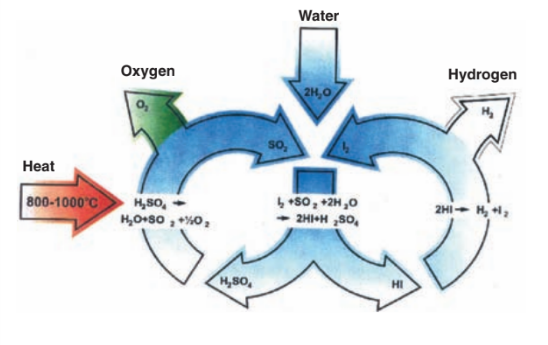
\includegraphics[width=0.4\linewidth]{figures/iodine-sulfur.png}
	\hfill
	\caption{Production of hydrogen by iodine-sulfur themochemical cycle.}
	\label{fig:isulfur}
\end{figure}

\section{HTGR Process Heat Application}

One of R\&D projects for the high tmeperature gas-cooled reactor is to develop more efficient energy conversion cyclse. The gas turbine/steam turbine (GS-ST) combined cycle is a practicable approach to imporve the HTGR energy conversion efficiency.

The HTR-10 design features allow it to accept a gas/gas intermediate heat exchanger in series with the steam generator, which gives the HTR-10 flexibility for multi-aspect applications. Fig. \ref{fig:gtst} shows the conceptual flow scheme of the GT-ST combined cycle for the HTR-10.

With adoption of the IHX and double cycles, the economic competitiveness is decreased and the system operation and control are more complex.

\cite{yuanhui_htgr_1996}

\begin{figure}[H]
	\centering
	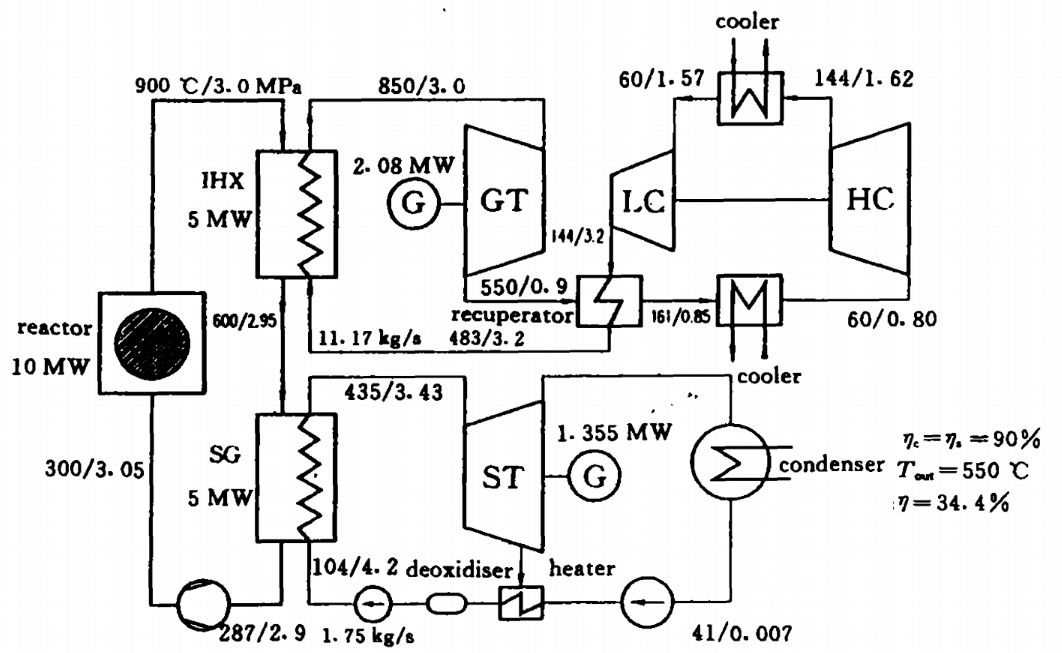
\includegraphics[width=0.4\linewidth]{figures/htgr-gtst.png}
	\hfill
	\caption{Gas Turbine/Steam Turbine (GT-ST) combined cycle in HTR-10.}
	\label{fig:gtst}
\end{figure}
